% !Rnw weave = Sweave
\documentclass[xcolor={table}]{beamer}


\RequirePackage{../assets/pres-template_MOW}
\usepackage[noae]{Sweave}
\usepackage{colortbl}

%--------------------------------------------------------------------------
% Specific to this document ---------------------------------------


%--------------------------------------------------------------------------
% \setbeamercovered{transparent}

%%%%%%%%%%%%%%%%%%%%%%%%%%%%%%%%%%%
\setlength{\tabcolsep}{1.3pt}
\title{PLSC 40601}
\subtitle{Week 7: Reviewing advances estimating techniques building on semiparemtric theory: DML/TMLE.}
\date{Spring 2023}
\author{Molly Offer-Westort}
\institute{Department of Political Science, \\University of Chicago}


\begin{document}
\input{plsc40601_slides_72-concordance}



%-------------------------------------------------------------------------------%
\frame{\titlepage
\thispagestyle{empty}
}
%-------------------------------------------------------------------------------%
\begin{frame}{Housekeeping}

\begin{wideitemize}
\item ?
\end{wideitemize}

\end{frame}


%%%%%NOTE%%%%%
\note{
\scriptsize \singlespacing

\begin{wideitemize}
\item xxxx
\end{wideitemize}

}

%-------------------------------------------------------------------------------%
% \begin{transitionframe}
% \centering
% 
% \LARGE \textcolor{white}{Trees}
% 
% \end{transitionframe}
% 
%-------------------------------------------------------------------------------%
\begin{frame}{Objective}

\begin{wideitemize}
\item Get point estimates, confidence intervals for a (potentially causal) low-dimensional parameter $\theta_0$ in the presence of high-dimensional nuisance parameters, $\eta_0$.\pause
\item $\eta_0$ may be so high-dimensional that traditional constraints on complexity of the parameter space, e.g., that estimators $\hat\eta$ lie in a space constrained by Donsker conditions,  break down. \pause (example: number of parameters grows with sample size)\pause
\item We would like to use machine learning methods to deal with the high-dimensional setting. 
\end{wideitemize}

\end{frame}


%%%%%NOTE%%%%%
\note{
\scriptsize \singlespacing

%\begin{itemize}
%\item xxx
%\end{itemize}
}
%-------------------------------------------------------------------------------%
\begin{frame}{ML methods}

\begin{wideitemize}
\item ML methods relax reliance on assumptions about functional form; \pause particularly useful with high dimensional data based on e.g., interactions, where we might not have strong substantive motivations for specific form. \pause
\item ML methods good at using regularization to reduce variance \pause $\rightarrow$ good performance on prediction. \pause
\item Good prediction does not imply good performance for estimation and inference, particularly for causal parameters.\pause
\item ML allows us to trade-off bias for variance, but we are not doing so optimally for the causal parameter we care about. 
\end{wideitemize}

\end{frame}


%%%%%NOTE%%%%%
\note{
\scriptsize \singlespacing

%\begin{itemize}
%\item xxx
%\end{itemize}
}
%-------------------------------------------------------------------------------%
\begin{frame}{DML Solution}

\begin{enumerate}
\item use Neyman-orthogonal scores that are less sensitive wrt nuisance parameters to estimate $\theta_0$\pause
\item use cross-fitting to deal with additional bias from ML estimators
\end{enumerate}

\end{frame}


%%%%%NOTE%%%%%
\note{
\scriptsize \singlespacing

%\begin{itemize}
%\item xxx
%\end{itemize}
}
%-------------------------------------------------------------------------------%
\begin{frame}{Overview of algorithm (DML2)}

\begin{enumerate}
\item Partition data into K equal folds \pause(4-5 seems good). \pause 
\item  Estimate nuisance parameters on each fold $k$, using appropriate ML estimators for the context. \pause (lots of sparsity? $\rightarrow$ lasso. Well approximated by trees? $\rightarrow$ random forest. And/or use ensemble methods.) \pause 
\item Estimate $\hat \theta_0$ as the solution to:
\[
\frac 1 K \sum_{k = 1}^K \E_{n, k} [\psi(W, \hat \theta_0, \hat \eta_{0,k})] = 0
\]
where $\psi$ is the Neyman orthogonal score, $\E_{n, k}$ is empirical expectation over $k$-th fold of the data, $W$ is a random element that takes values in a measurable space. 

\end{enumerate}

\end{frame}


%%%%%NOTE%%%%%
\note{
\scriptsize \singlespacing

%\begin{itemize}
%\item xxx
%\end{itemize}
}
%-------------------------------------------------------------------------------%
\begin{frame}{TMLE Solution}

DML approach might produce results that perform well asymptotically, but don't have nice small sample properties. \pause

\begin{enumerate}
\item Estimate the density using some estimating model that will have nice behavior \pause 
\item Then update in the model space, avoiding predictions that will be outside the density of the data / parameter space. 
\end{enumerate}

\end{frame}


%%%%%NOTE%%%%%
\note{
\scriptsize \singlespacing

%\begin{itemize}
%\item xxx
%\end{itemize}
}
%-------------------------------------------------------------------------------%
\begin{frame}{Overview of algorithm (Focusing on ATE)}

\begin{enumerate}
\item Split the data into folds. \pause Within a given training + validation pair:\pause
\item Generate initial estimate of conditional mean outcome $\hat Y_A = \hat \E [Y | A, \X ]$ on training data. \pause 
\item Generate estimate of exposure mechanism, $\hat\pi_a = \hat P[A = a | \X]$. \pause
\item Update initial estimate of $\hat \E [Y | A, \X ]$ on validation data.\pause
\begin{itemize}
\item Calculate $H_a(A = a, \X) = \frac{\mathbbm{I}(A = 1)}{\hat \pi_1} - \frac{\mathbbm{I}(A = 0)}{\hat \pi_1}$\pause
\item Regress $Y$ on $H_a$, specifying $\hat Y_a$ as offset. \pause
\item Generate counterfactual predictions from this new regression model, $\hat Y_1^*, \hat Y_0^*$. \pause
\end{itemize}
\item 
Averaging across folds:
\[
\hat{\theta}_{\textrm{CV-TMLE}} = \frac 1 K \sum_{k = 1}^K \E_{n, k}\left[\hat Y_1^{k*} - \hat Y_0^{k*} \right]
\]
\end{enumerate}\pause

Technically you can do TMLE without machine learning OR crossfitting. 

\end{frame}


%%%%%NOTE%%%%%
\note{
\scriptsize \singlespacing

%\begin{itemize}
%\item xxx
%\end{itemize}
}
%-------------------------------------------------------------------------------%
\begin{frame}{Cross-fitting}

\begin{figure}
\centering
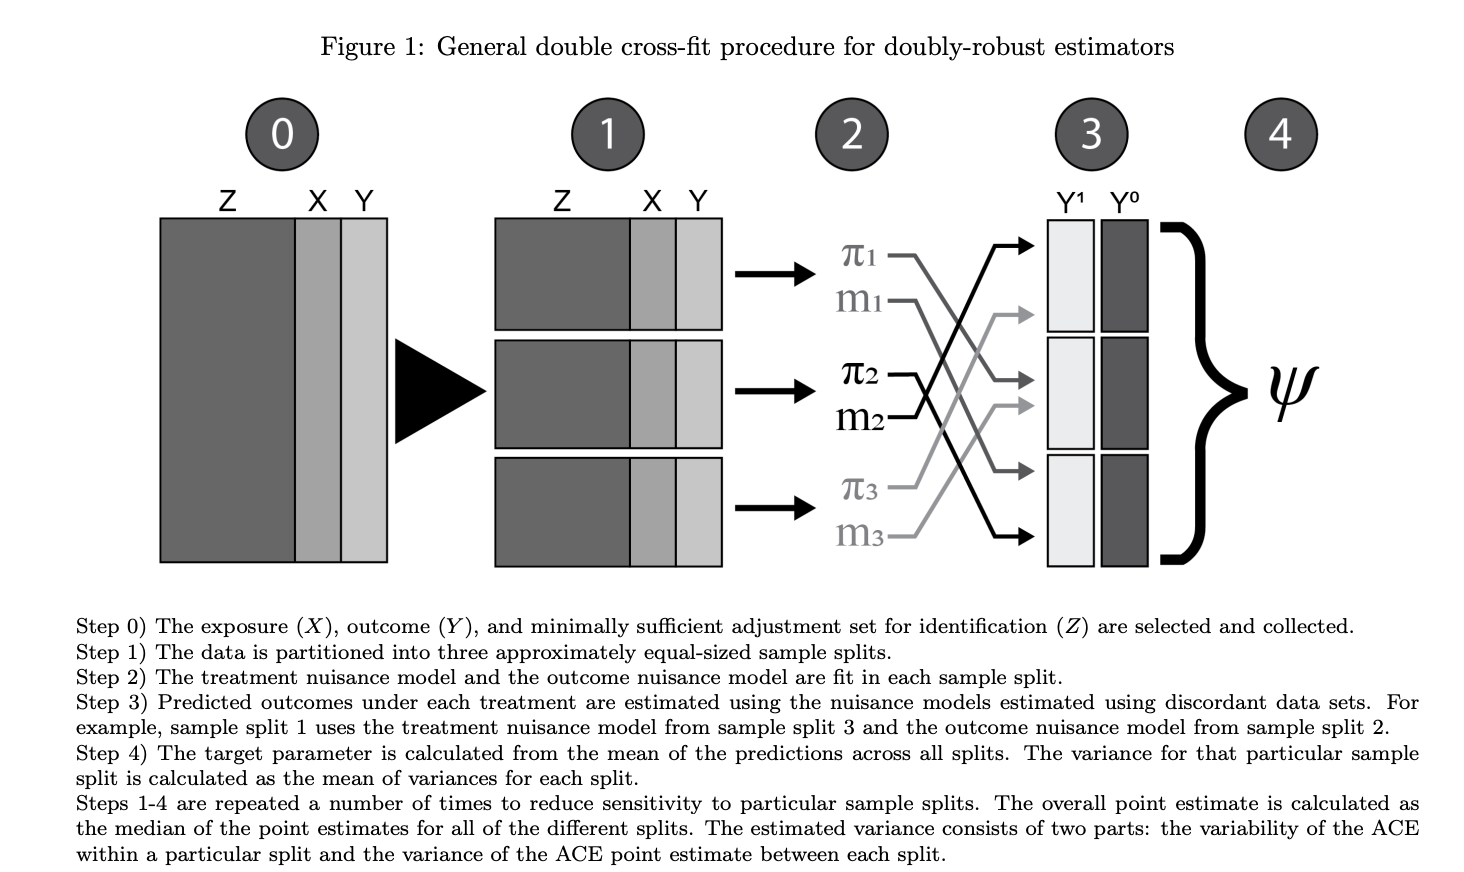
\includegraphics[width = 0.8\textwidth]{../assets/zivich-breskin_cv.png}
\end{figure}
\hfill \cite{zivich2021machine}
\end{frame}

%%%%%NOTE%%%%%
\note{
\scriptsize \singlespacing

\begin{wideitemize}
\item xxxx
\end{wideitemize}

}

%-------------------------------------------------------------------------------%
\begin{frame}{Cross-fitting}

\begin{wideitemize}
\item As with DML, there are some different approaches to cross-fitting; e.g., updating step can be pooled across folds. 
\end{wideitemize}

\end{frame}


%%%%%NOTE%%%%%
\note{
\scriptsize \singlespacing

\begin{wideitemize}
\item xxxx
\end{wideitemize}

}

%-------------------------------------------------------------------------------%
\begin{frame}{Relative benefits of TMLE vs. DML}

\begin{figure}
\centering
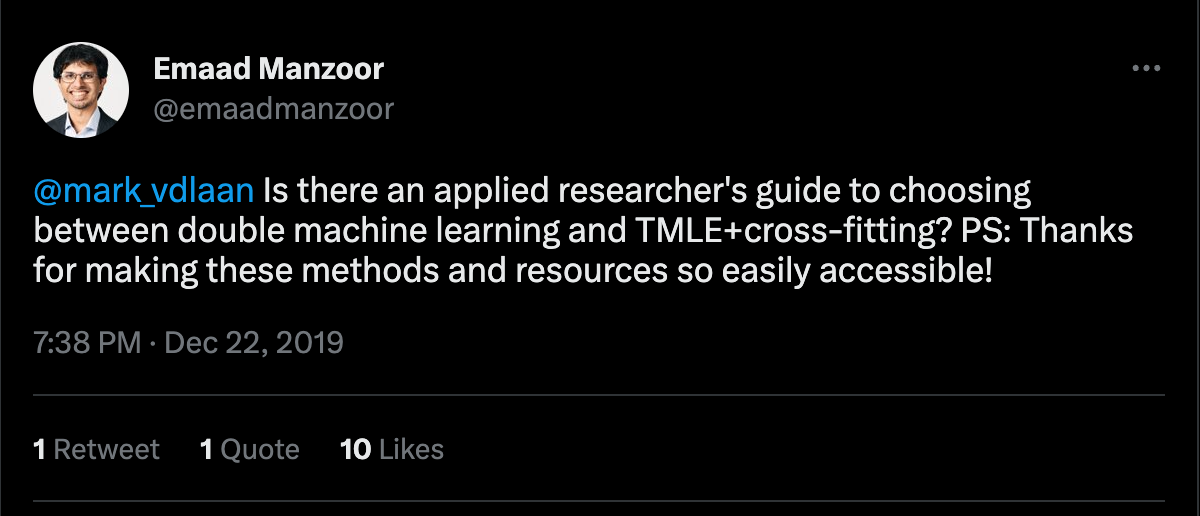
\includegraphics[width = 0.8\textwidth]{../assets/tmle-dml-empirical-tweet.png}
\end{figure}
\hfill
\end{frame}


%%%%%NOTE%%%%%
\note{
\scriptsize \singlespacing

\begin{wideitemize}
\item xxxx
\end{wideitemize}

}
%-------------------------------------------------------------------------------%
\begin{frame}{Relative benefits of TMLE vs. DML}
Response: \url{https://vanderlaan-lab.org/2019/12/24/cv-tmle-and-double-machine-learning}\pause

Some arguments: \pause
\begin{wideitemize}
\item TMLE ``respects'' constraints of the model, especially useful with, e.g., rare outcomes \citep{balzer2016estimating}\pause
\item No issues with multiple solutions\pause
\item ``We also note that the TMLE is the only estimator that actually generalizes the MLE – if the MLE is well-defined and used as initial estimator, then the TMLE is exactly equivalent to the MLE (i.e., the targeting step will select zero fluctuation).'' 
\end{wideitemize}

\end{frame}


%%%%%NOTE%%%%%
\note{
\scriptsize \singlespacing

\begin{wideitemize}
\item xxxx
\end{wideitemize}

}

%-------------------------------------------------------------------------------%
\begin{frame}{Application to data}
\cite{zivich2021machine}

\begin{figure}
\centering
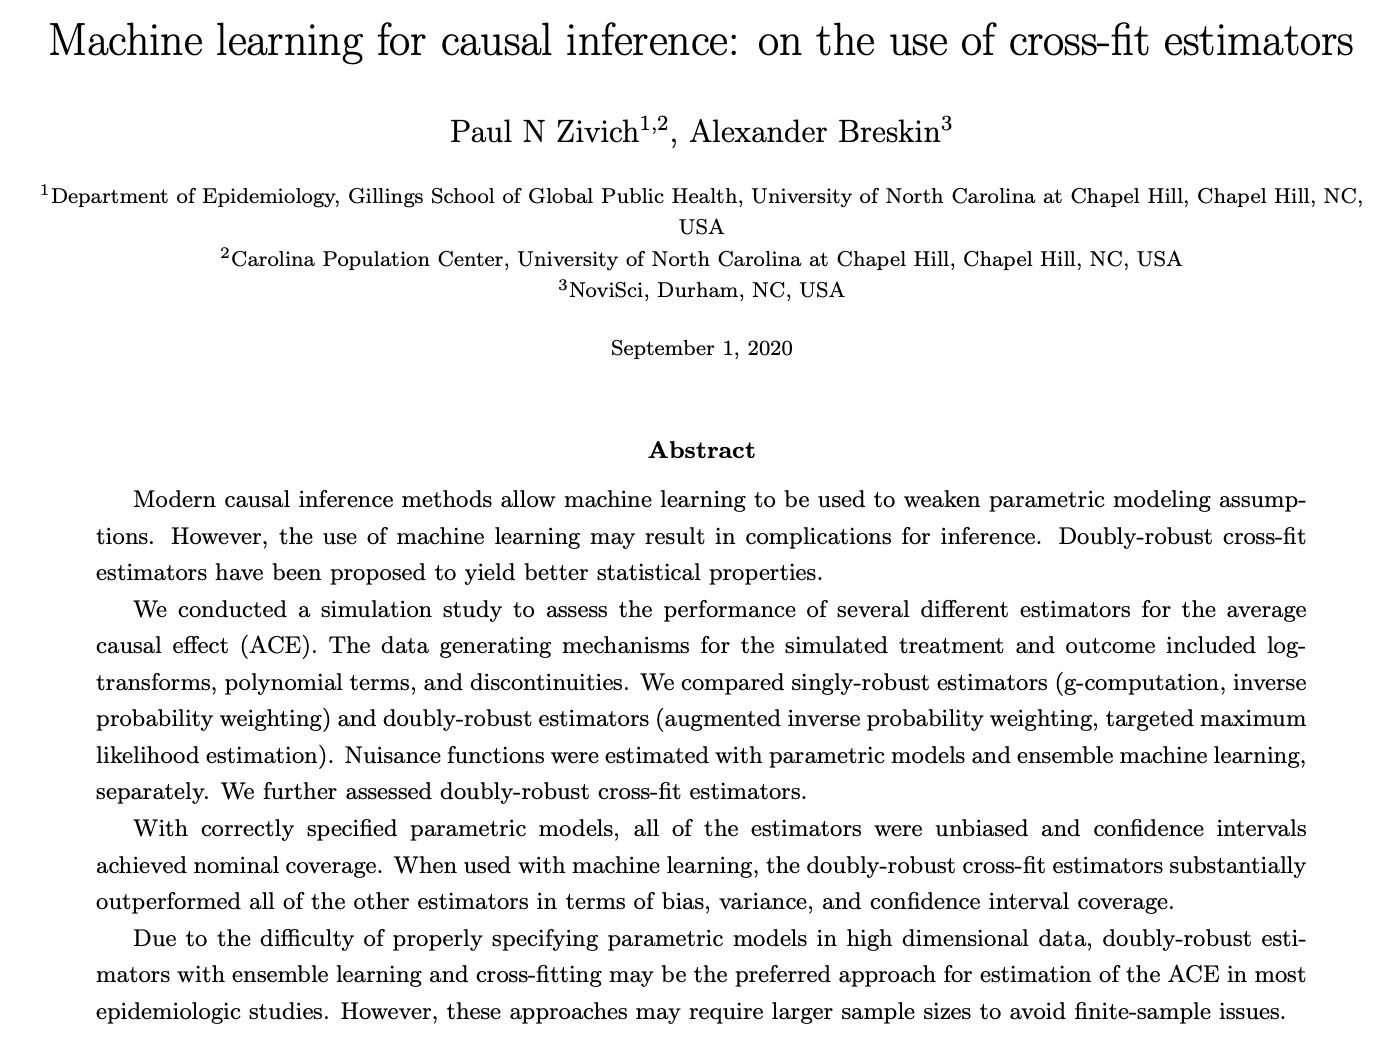
\includegraphics[width = 0.8\textwidth]{../assets/zivich-breskin.png}
\end{figure}
\hfill
\end{frame}


%%%%%NOTE%%%%%
\note{
\scriptsize \singlespacing

\begin{wideitemize}
\item xxxx
\end{wideitemize}

}

%-------------------------------------------------------------------------------%
\begin{frame}{Application to data}
\cite{zivich2021machine}

\begin{figure}
\centering
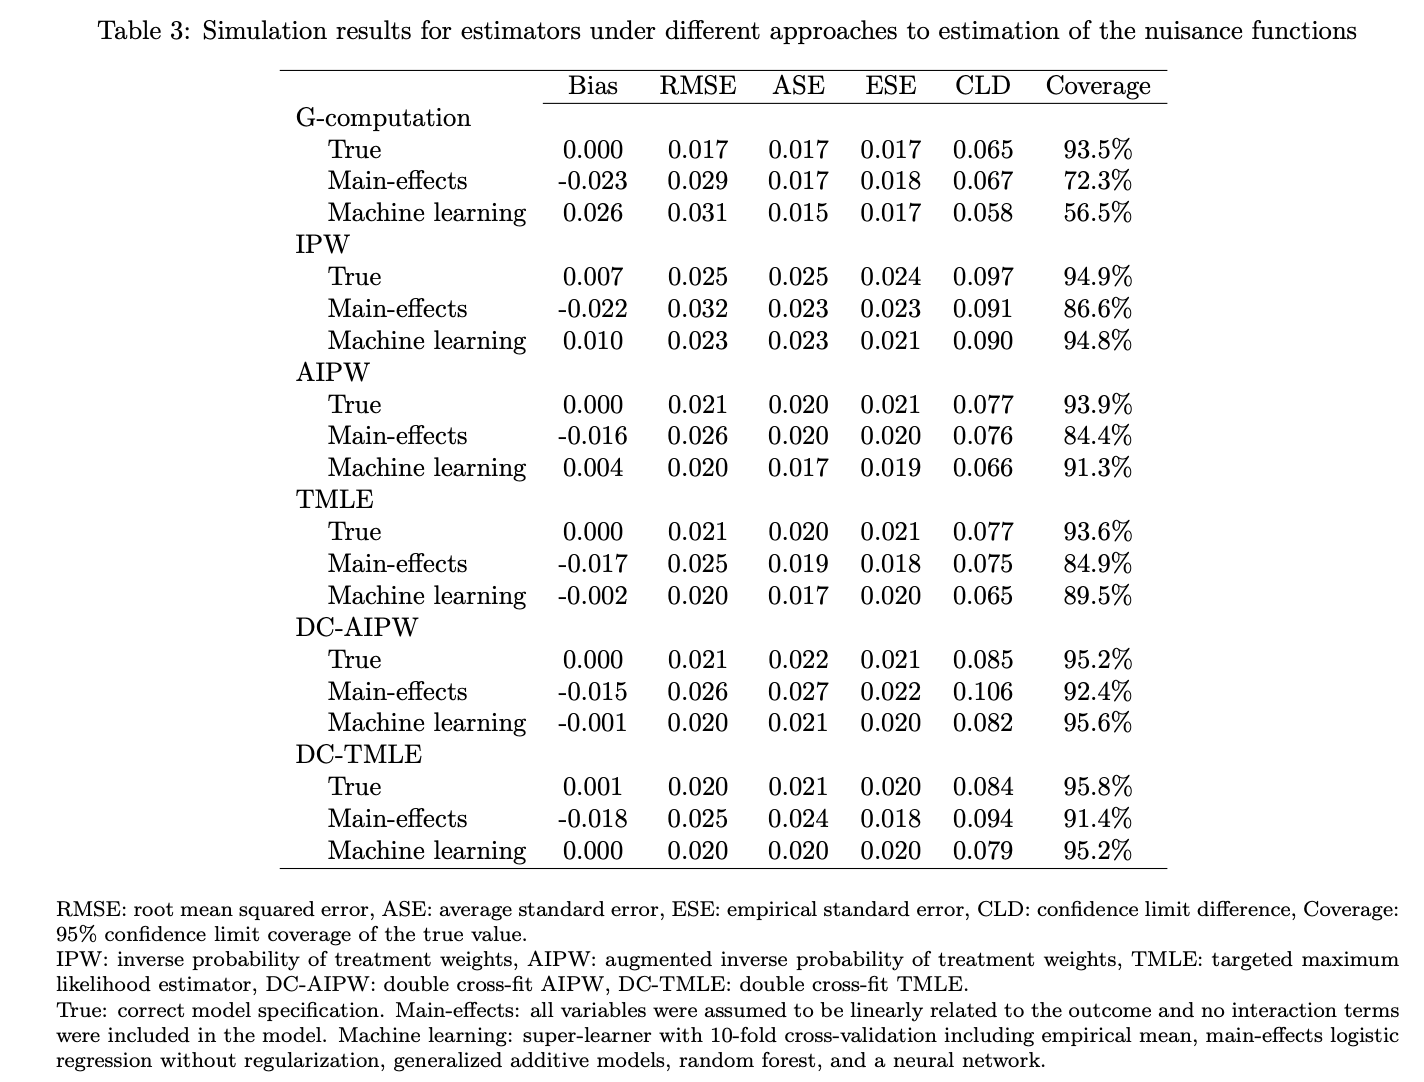
\includegraphics[width = 0.8\textwidth]{../assets/zivich-breskin_table3.png}
\end{figure}
\hfill
\end{frame}


%%%%%NOTE%%%%%
\note{
\scriptsize \singlespacing

\begin{wideitemize}
\item xxxx
\end{wideitemize}

}

%-------------------------------------------------------------------------------%
\begin{frame}{The goal}

\begin{wideitemize}
\item Estimation of a causal parameter\pause
\begin{itemize}
\item unbiased\pause
\item consistent\pause
\end{itemize}
\item Possible sources of bias\pause
\begin{itemize}
\item identification
\item estimation\pause
\end{itemize}
\item Possible uses of covariates\pause
\begin{itemize}
\item Required for causal model
\item Covariate adjustment for precision 
\end{itemize}
\end{wideitemize}

\end{frame}


%%%%%NOTE%%%%%
\note{
\scriptsize \singlespacing

\begin{wideitemize}
\item xxxx
\end{wideitemize}

}

%-------------------------------------------------------------------------------%


\backupbegin
%-------------------------------------------------------------------------------%

\nocite{schuler2017targeted,chernozhukov2018double}
\begin{frame}[allowframebreaks]{References}
    \bibliographystyle{apalike}
    \bibliography{../assets/PLSC40601}
\end{frame}
%-------------------------------------------------------------------------------%
\backupend
\end{document}
%
%-------------------------------------------------------------------------------%
%%% [[TEMPLATE]] %%%
\begin{transitionframe}
\centering

\LARGE \textcolor{white}{Statement.}

\end{transitionframe}
%-------------------------------------------------------------------------------%

%%% [[TEMPLATE]] %%%
\begin{frame}{Frametitle}

\begin{wideitemize}
\item xxx
\end{wideitemize}

\end{frame}


%%%%%NOTE%%%%%
\note{
\scriptsize \singlespacing

\begin{wideitemize}
\item xxxx
\end{wideitemize}

}

%-------------------------------------------------------------------------------%
